\documentclass[continuous]{grattan}
\usepackage{layout}
\usepackage{blindtext}

\title{Report title}
\author{author and author}

\MONTH{October}  % If omitted, these take the date of compilation
\YEAR{2016}
\GrattanReportNumber{2016-X}

\addbibresource{AP-bibliography.bib}
\addbibresource{bibtester.bib} % for long-url

\listfiles

\begin{document}
\layout
\contentspage

\listoffigures

\begin{overview} 
A federal election is an opportunity to take stock of how Australia
is doing, where it’s going, and what governments can do about it.
This report surveys policy recommendations from seven years of
Grattan Institute reports and outlines what the Commonwealth
Government should do to improve Australia.

The problems aren’t hard to find. Per capita national income has
fallen over the last four years as the mining boom subsided.
Economic growth is slow, reflecting trends across the developed
world. Unemployment stands at nearly six per cent, higher than in
the United States and United Kingdom, countries hit much harder
by the Global Financial Crisis than Australia. Underemployment
also remains high.

Commonwealth budgets haven’t come close to balancing for eight
years. Interest on the accumulating debt now consumes 4 per
cent of government income, or as much as the Commonwealth
spends on public hospitals. Younger generations will be taxed
more to pay for today’s spending. Every \$40 billion deficit, the
norm for each of the last eight years, forces households aged 25
to 34 to pay an extra \$10,000 in tax over their working lives.
Our large capital cities have growing pains. House prices are very
high relative to incomes. Home ownership is falling for all
households aged under 55. Most new housing is far from the city
centres where most new jobs are being created. More people
spend longer in traffic getting to work. The physical divide
between rich and poor is growing.

School education is not keeping up with the best in the world. Test
results are well behind international benchmarks, and Australia is
slipping down global rankings. Between Years Three and Nine,
talented students from poorer backgrounds fall almost two years
behind their peers from richer backgrounds.

Our political system is not dealing well with these challenges.
Politicians are often creating great expectations that far exceed
what government can ever do. Meanwhile, they are failing to act
on the things that they can control. The result is an often barren
debate that disappoints everyone and makes for a dull campaign.
Yet there are many reforms that can contribute to economic
growth, improve the quality and reduce the cost of government
services, and bring budgets back into balance. A growing
evidence base shows which reforms would work.

Progress on this agenda has been underwhelming for a decade,
perhaps because the prosperity of the mining boom sapped the
will for reform. The politics of reform is never easy. Vested interest
groups, emboldened by success, are more vocal in protecting
their interests. Meanwhile the public interest has few friends.
Ironically, though, the public seems to be up for reform. Surveys
suggest that people understand the need for budget repair, and
are even prepared to contemplate slaying sacred cows such as
negative gearing.

Our politics can implement this reform agenda by using the
evidence that has been assembled, robustly articulating the public
interest, and staring down interest groups. Australia has a proud
history of enlightened public policy. Many countries would be
delighted to swap our problems for theirs. Australia can continue
to be the lucky country. But we must make our own luck.
\end{overview}

\chapter{Economic growth priorities}
\begin{verysmallbox}[H]{Summary}{box:economic-growth-priorities}
Improving the efficiency of Australian taxes could provide a big
kick to economic growth. In particular, the Commonwealth should
encourage the States to replace stamp duties by general property
taxes.

Lifting workforce participation rates for women and older workers
could boost economic growth, and counter the ageing of the
workforce. The Commonwealth should ask the Productivity
Commission to assess combinations of tax, transfer, and
childcare support that would reduce welfare traps and encourage
higher female labour force participation for a given budgetary
cost. The Commonwealth should also raise the age of access to
the Age Pension and superannuation to 70 years.

Government should remove inappropriate impediments to
flexibility in the economy, so that resources can be swiftly
reallocated to their highest value uses as conditions change.
Government should remove barriers to innovation, but should not
waste money in its name. Removing barriers to the local spread of
global innovations is likely to make more difference to economic
growth than subsidies for Australian inventions.

With many of the economy-wide reforms already completed,
industry-specific reforms – especially in sectors such as
superannuation – may well comprise the bulk of the productivity
increases that government reform can achieve.
\end{verysmallbox}

\section{Scope}
This report aims to help the next Commonwealth Government to
set priorities for reform. Drawing primarily on work published by
Grattan Institute over the last seven years, it identifies policy
changes that the Government should adopt to make the most
difference to the lives of Australians.

The report considers reforms to increase economic growth and
reduce budget deficits. It discusses reforms to policy for tax and
budgets, cities, transport, energy, school education, higher
education and health. Grattan Institute has focused on these
because they make a big difference to the lives of Australians,
because analysis can chart a path to better policy, and because
outcomes are too often driven by vested interests rather than the
public interest.

The report does not cover areas such as foreign affairs and trade,
immigration, defence and security, law and order, industrial
relations, communications, human services, indigenous affairs
and the environment. These areas matter, but have not been part
of Grattan Institute’s work to date.

The report focuses on issues that the Commonwealth can
influence directly rather than those that are essentially State
responsibilities. It selectively identifies areas where there might be
a clear rationale for the Commonwealth to make additional tied
grants to the States.\footnote{In this report, “States and Territories” are abbreviated to “States”.} 
These areas include situations where the Commonwealth budget would substantially benefit from State
Government reforms.


\section{Spending projections}
The Commonwealth’s spending projections also seem optimistic. They assume tight spending restraint, with government spending falling as a share of the economy (\Cref{fig:FISCAL-2}).\footcite[][5--11]{Treasury2015BudgetPapers201516}  The projections forecast spending to grow at just 2.6~per cent a year on average between 2014\nobreakdash-15 and 2025\nobreakdash-26, far below the 3.6~per~cent average growth rate of the last decade.\footcite[][5]{PBO2015}  Consistent with this spending restraint, the Commonwealth Government forecasts that spending will decline to 24.2 per cent of GDP in 2024-25, below its long term average.\footcite[][3--9]{Treasury2015BudgetPapers201516}  

Spending is forecast to be below the historical average in all program areas other than defence, as is shown in \Vref{fig:FISCAL-8}, which compares the projected growth in the Commonwealth’s largest spending programs over the next 10 years with the history of the last 10~years. 

\begin{figure}
\caption{Spending forecasts rely on lower growth in almost all major programme areas\label{fig:FISCAL-8}}%
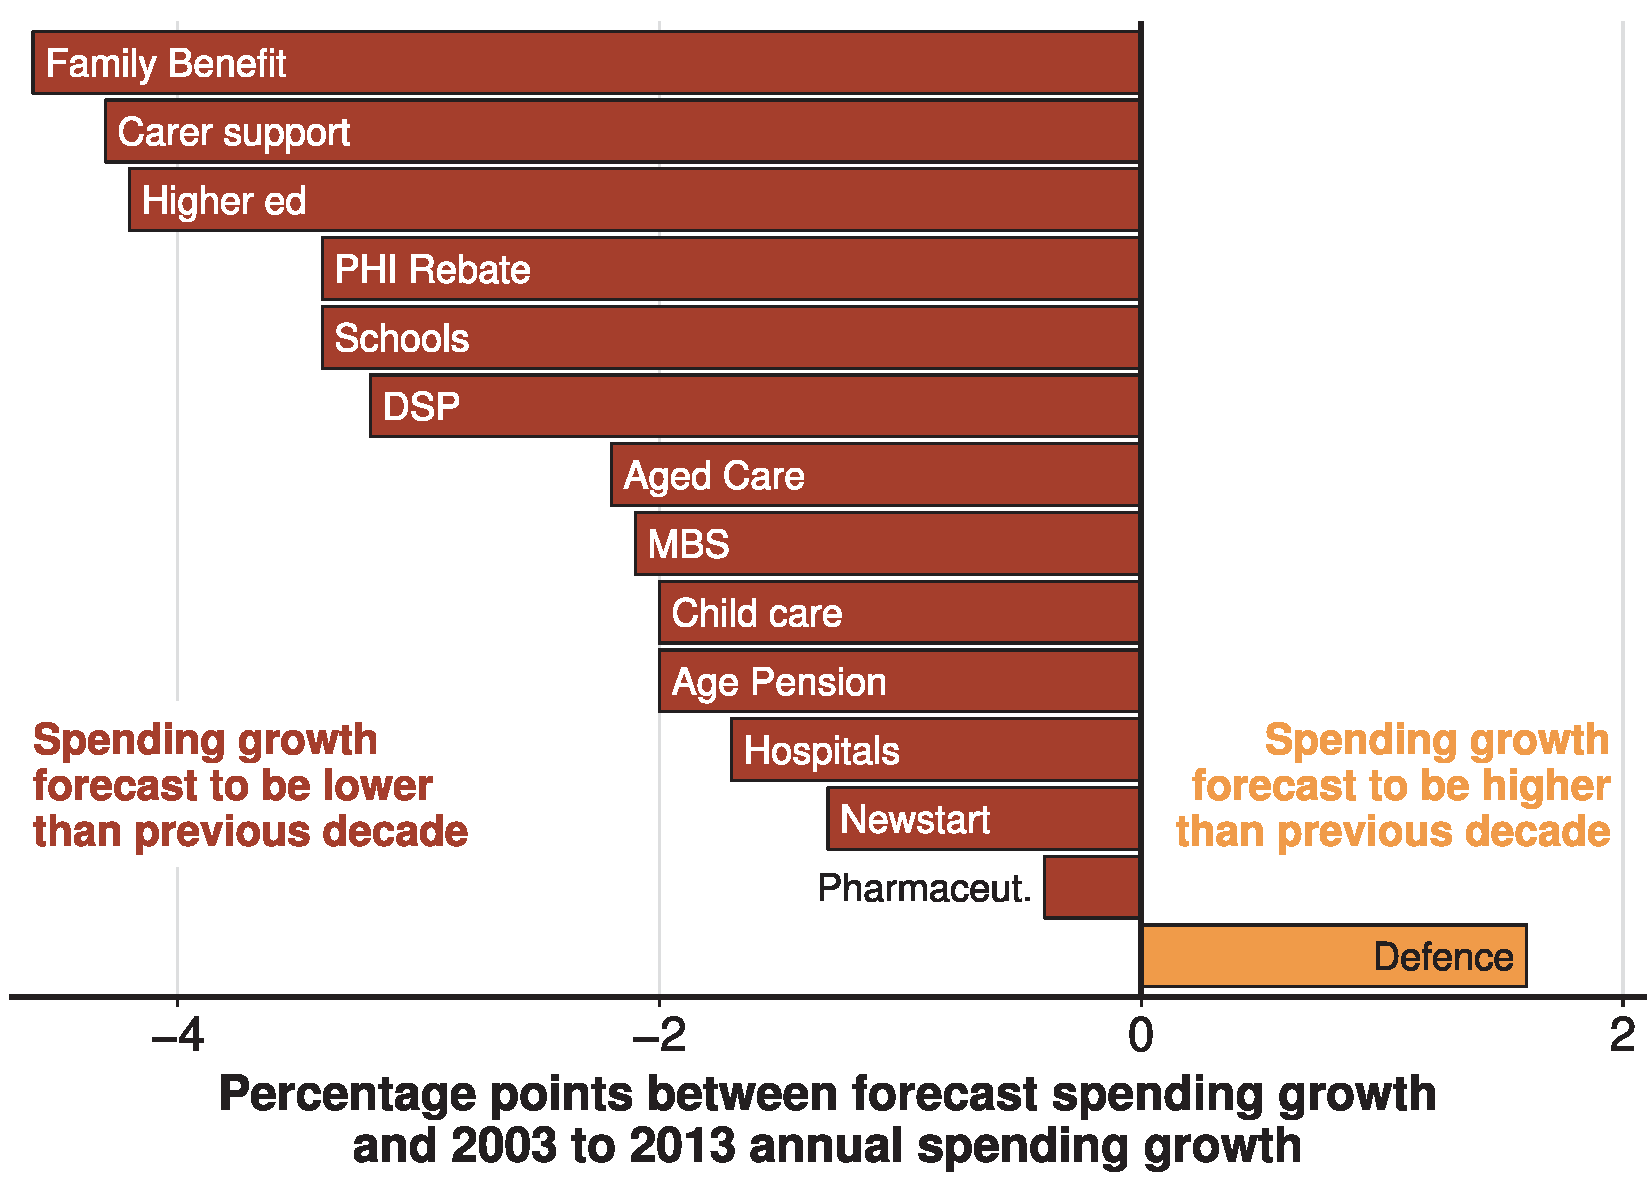
\includegraphics[width=\columnwidth]{figure/budget-repair-Figure8-altered-1.pdf}
\noteswithsource{The defence estimates do not factor in the commitment to increase defence spending to 2~per~cent of GDP by 2023-24. Rather they are based on the long-term funding commitments made in previous Defence White Papers and government announcements.}{{\textcite{PBO2014}}}
\end{figure}

Some of these estimates seem improbable. For example, it seems unlikely that spending on demand-driven programs such as the \textbf{Medicare Benefits Schedule} will moderate without significant policy changes. The PBO attributes the strong historical growth in Medicare payments to policies (such as the Bulk Billing Incentive and the Extended Medicare Safety Net) that have made Medicare services more attractive or accessible. New policy measures such as the freeze in Medicare scheduled fees are forecast to produce lower growth. Yet for more than 20 years the ageing of the population, medical science and technology improvements and rising expectations of the health system have put relentless pressure on the health budget.\footcite{Daley2014}  These pressures will not abate, and the forecasts almost certainly understate them.

The decline in spending growth for hospitals and schools may be credible given the decision in the 2014-15 Budget to limit spending increases to inflation and population growth. This of course does not mean that spending growth will decline in these program areas – merely that the states will have to bear all of the cost of real per capita growth.

The 2015-16 budget assumes even tighter spending growth than have previous budgets. Except for welfare spending, mainly driven by the NDIS, no category is expected to grow materially faster than inflation.\footcite[][BP No.~1, pp.\ppspace 5--11]{Treasury2015BudgetPapers201516}  

In other programs, lower forecast growth rates are tied to measures from the 2014-15 and 2015-16 Budgets that are unlikely to be passed by the Senate. Therefore spending on the Carers Payment, higher education and Newstart benefits is likely to be more than forecast. Even the forecast growth in defence spending – the only program area where spending is forecast to grow faster than in the last decade – does not put Australia on a path to spend 2~per~cent of GDP on defence by 2023-24 as the Government has promised.\footnote{See: \textcite[][1]{Defence2014}.} 


Spending projections also assume there will be no new spending initiatives promised at elections or in response to natural disasters or community demands for more assistance to the disadvantaged. Experience over the last decade suggests that such spending restraint will be difficult (\Vref{box:FISCAL-1}).

Given all the number of things that need to go right, moderating spending growth to 24.2~per~cent of GDP in 2024-25 seems extremely unlikely without further explicit budget measures to cut expenditure.


\begin{table}
\captionwithunits{Approaches to valuing properties for council rates vary\label{tbl:PROP-1}}%
{Property value bases that can be used to set council rates in each state}
\begin{tabularx}{\columnwidth}{>{\bfseries}lX}
%
\toprule
\textbf{State} & \textbf{Basis for council rates} \\%[0.5\baselineskip]
\midrule
\textbf{NSW}   & Unimproved  \\[0.5\baselineskip]
\textbf{QLD}   & Unimproved  \\[0.5\baselineskip]
\textbf{VIC}   & Either unimproved or capital improved  \\[0.5\baselineskip]
\textbf{WA}    & Capital improved  \\[0.5\baselineskip]
\textbf{SA}    & Either unimproved or capital improved \\[0.5\baselineskip]
\textbf{TAS}   & Either unimproved or capital improved  \\[0.5\baselineskip]
\textbf{NT}    & Unimproved  \\[0.5\baselineskip]
\textbf{ACT}   & Unimproved  \\%[0.5\baselineskip]
\bottomrule
\end{tabularx}
\noteswithsource{‘Unimproved’ refers to a set of land valuations that capture the value of the land only. ‘Capital improved’ refers to valuations that capture the value of the land and significant capital improvements made to that land, such as buildings.}{%
\mbox{\textcites{productivity2008assessing}{mangioni2014re}{Treasury2014-Interstate-Comparison-Taxes1415}}.}
\end{table}

\begin{bigbox*}{Impact of limiting negative gearing {and CGT} tax concessions on house prices}{box:ImpactOfPrice}

We model the impact of our policy proposal detailed in chapter 5: quarantining rental loss deductions and reducing the CGT discount to 25~percent. Other reforms would have different effects, although they are likely to be similar order of magnitude.

Two different approaches yield similar results. Firstly we calculate the capitalised value of the revenue foregone from the tax changes as a percentage of total residential property value. Secondly, we calculate the change in return as a proportion of property value, and as a proportion of all property owners



The proposed changes to negative gearing would reduce tax write-offs for property investment by about \$2~billion initially and \$1.7~billion over time. Assuming a discount rate of 
5~percent, the present value of these lost tax benefits would be approximately \$34.3~billion.


The proposed reduction of the capital gains tax discount to 25~percent would reduce after tax returns by about \$3.65~billion a year, or \$73.1~billion in perpetuity. Assuming 40~percent of this relates to gains on real estate (in line with 2013-14 gains realisations) then the expected present value of the lost benefits for would be approximately \$29.2~billion.



If these lost benefits (\$29.2~billion + \$34.3~billion) were fully capitalized into the value of residential property -- currently worth \$5.4~trillion -- prices would fall in the order of 1.1~percent.

\eject
\begin{table}[H]
\captionsetup{labelfont = {small, bf, theGrey}, position=above, aboveskip=-1pt, font = {small, theGrey}} % 1pt magical for baseline alignment with first column
\caption{Impact of policy changes on after-tax returns}\label{tbl:Impact-house-prices}
\makebox[\linewidth][c]{

% latex table generated in R 3.2.5 by xtable 1.8-2 package
% Sun Apr 24 12:04:39 2016
\newcolumntype{R}{>{\raggedleft\arraybackslash}X}
\begin{tabularx}{\linewidth}{lRRRR}
  \toprule
   &  & \multicolumn{3}{c}{\textbf{Return}}\\
 \cmidrule(lr){3-5}
\textbf{Owner type} & {\textbf{Share of property}} & \textbf{BAU} & \textbf{Proposed} & \textbf{\ensuremath{\Delta} \%}\\
 \midrule
Negatively geared   & 18.0\%                     & 7.0\%        & 6.5\%             & 6.1\% \\
Positively geared   & 7.0\%                      & 6.4\%        & 6.0\%             & 6.8\% \\
Ungeared            & 5.0\%                      & 5.8\%        & 5.3\%             & 7.8\% \\
Owner-occupied      & 70.0\%                     & -            & -                 & - \\
   \bottomrule
\end{tabularx}


}

\notes{Negatively geared property had 80\%\ of the value of the property borrowed; positively geared is 40\%.}
\end{table}
\vspace*{-11pt}  % cosmetic

Alternatively, we can calculate the impact of tax changes on returns as a proportion of asset values for different classes of owners as shown in
\Vref{tbl:Impact-house-prices}.

Weighting these changes in returns by the share of residential property, suggests the average return (and therefore the price) would fall by about 2~percent. Yet this somewhat overstates the overall price effect because it is based on the change in returns for a representative investor in the top (47 per cent) tax bracket.

Of course, price changes would not be uniform. Prices would fall by more in the segments of the market with more investors (inner city apartments, for example). The change in returns for investors indicates the \emph{maximum} rational price change (about 7.4~per cent). However, this would only occur in locations where every prospective purchaser was an investor, and the fall in prices did not attract any owner occupiers. Tax changes would be unlikely to drag on property prices in any location by more than 3--4 per cent.

\end{bigbox*}

\chapter{Capital gains tax and asset lock-in}\label{appendix:CGT-asset-lock-in}
One reason often provided for lower taxes on capital gains is to reduce ``asset lock-in''. If investors are less likely to realise gains when tax rates are higher than increasing taxes on gains could actually reduce tax collections in the short to medium term. But the empirical evidence of lock-in in not settled. In Australia, the primary driver of asset lock-in appears to be people waiting until retirement to sell their assets. This incentive is still strong even with a 50 per cent discount. 

\section{Why does asset lock-in occur?}
Asset lock-in occurs because taxes are only paid when gains are realised. This provides an incentive for investors to hold on to assets with large accumulated gains.\footcite{Burman2009}  In effect, the investor seeks to maintain the implicit interest free loan on accrued gains. Crystallising a capital gain is only worthwhile if an investor can achieve a materially higher return elsewhere, or if they want the resources for consumption (\Vref{box:CGT-asset-lock-in}).\footcite[][12]{Ingles2009a}   

Lock-in can discourage investors from moving their money to the investments with the highest pre-tax returns, so assets do not always go to their highest value use.\footcite{Lindsey1987}  Lock-in effects are most significant from a whole of economy perspective, if they constrain financing of profitable investments.\footcites{OECD2006TaxationOfCapitalGains}{Johnson2008}  

\newcommand{\Act}[2]{\textit{#1} (#2)}
Australia’s open capital markets and generous capital gains tax regime for non-residents, reduce the danger that worthwhile projects will not get access to capital because of lock-in.\footnote{Non-resident investors in Australian shares are generally not subject to Australian capital gains tax (see: \Act{Income Tax Assessment Act 1936}{Cth}, s 136-25). } 


\begin{smallbox}[!hp]{Capital gains tax and asset lock-in}{box:CGT-asset-lock-in}
The tax treatment of capital gains can deter investors from taking up otherwise profitable investment opportunities. 



Suppose Hayley, an investor in the top tax bracket purchases a house for \$700,000 and holds it for 10 years. During that time the market price of the house increases to \$1,000,000. She makes a net rental return of 5~percent a year, so her  final income is \$50,000. 

If she were to sell the house she would crystallise the \$300,000 in gains, paying tax on 50~percent of the gains at her marginal tax rate of 49~percent (\$73,500). This would leave her with around \$926,500 from the sale: \$226,500 in net gains and her initial investment of \$700,000. 

The sale will only be worthwhile if Hayley can find an alternative property that yields more than her current rental income of \$50,000  with the same opportunity for capital gains. With her \$926,500 sale proceeds she would need to find a property with net rental return of more than 5.4~percent a year. 

Properties with rental yields below 5.4~percent but higher than her current 5 would not be attractive because realising the tax liability on her current property erodes her capital base for investment.  

The higher the tax rate on capital gains the less willing she will be to realise gains to pursue new investment opportunities. If capital gains were taxed in full, rather than with a 50 per cent discount, her hurdle rate for the new investment would be 5.9~percent.
\end{smallbox}

\begin{figure}%
\Caption{Pre-tax contributions of more than \$25,000 a year will likely be made mainly by high-income men}%
{Projected number of individuals in 2017-18 making pre-tax contributions of more than \$25,000}%
{fig:pre-tax-contributions-25k-by-decile-201718}
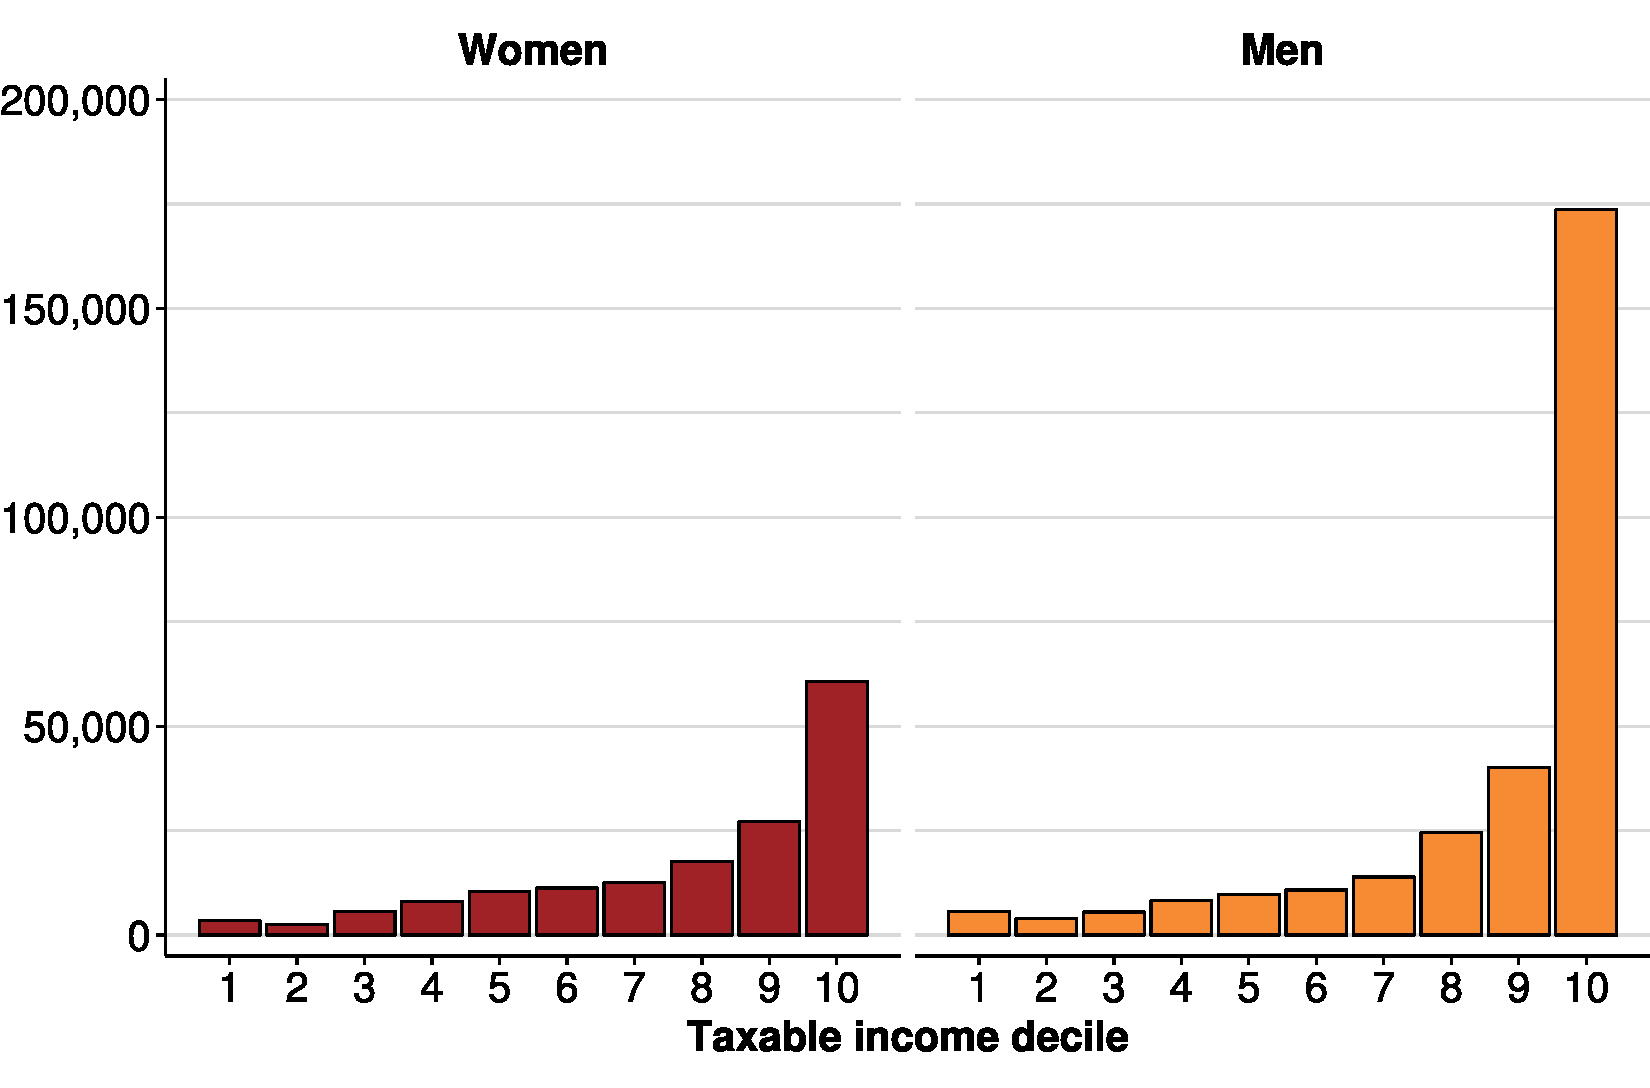
\includegraphics[width=4.47222in,height=2.94759954545455in]{figure/n-individuals-contr-over-25k-by-decile-201718-1} 
\noteswithsource{Pre-tax super contributions made by individuals in the ATO 2 per cent
sample file for 2013-14 are adjusted to reflect total pre-tax contributions reported
in ATO Taxation Statistics for superannuation funds, such as by estimating
Super Guarantee contributions for taxpayers with salary income but who report
no pre-tax contributions from their employer and accounting for people who do
not lodge their tax return on time. Contributions are then projected forward to
2017-18 to account for increases in nominal incomes and growth in the working
population. The range of taxable incomes included in each decile is the same for
men and women.}{%
Grattan analysis of \textcite{ATO2016SampleFile1314}.}
\end{figure}


\section{``Carry forward'' provisions are not needed}\label{sec:carry-fwd-provisions-not-needed}

While most of the Government’s proposed changes will better target contributions tax breaks, the “carry forward” provisions are a step backwards. 
The Government proposes that taxpayers with a super balance of less than \$500,000 will be able to draw on unused pre-tax caps from the previous five years to make ``catch-up'' contributions.
In theory, these provisions are supposed to help women, carers and others with broken work histories. 
The ALP does not support this change.\footcite{Bowen-2016-Labors-plan-for-super-not-retrospective}


Restricting the catch-up allowance to those with a balance of less than \$500,000 would exclude some people. 
But it does not materially improve the targeting: those likely to use the catch-up allowance will still mostly be men on higher incomes; 
only 11~per~cent would be women aged below~50.
A mere 1~per~cent of women with superannuation balances of less than \$500,000 -- 96,000~people -- are expected to make pre-tax contributions of \$25,000 or more in 2017-18.
Most~of them would be among the top 20 per cent of income earners (\Vref{fig:n-individuals-by-decile-over-500k-and-over-25k-201718}). %\enlargethispage*{0.5\baselineskip}

\begin{figure}%
\Caption{Allowing taxpayers to carry forward unused caps will mainly help wealthier men}%
{Projected number of individuals in 2017-18 with super balances of less than \$500,000 and making pre-tax contributions of at least \$25,000}%
{fig:n-individuals-by-decile-over-500k-and-over-25k-201718}

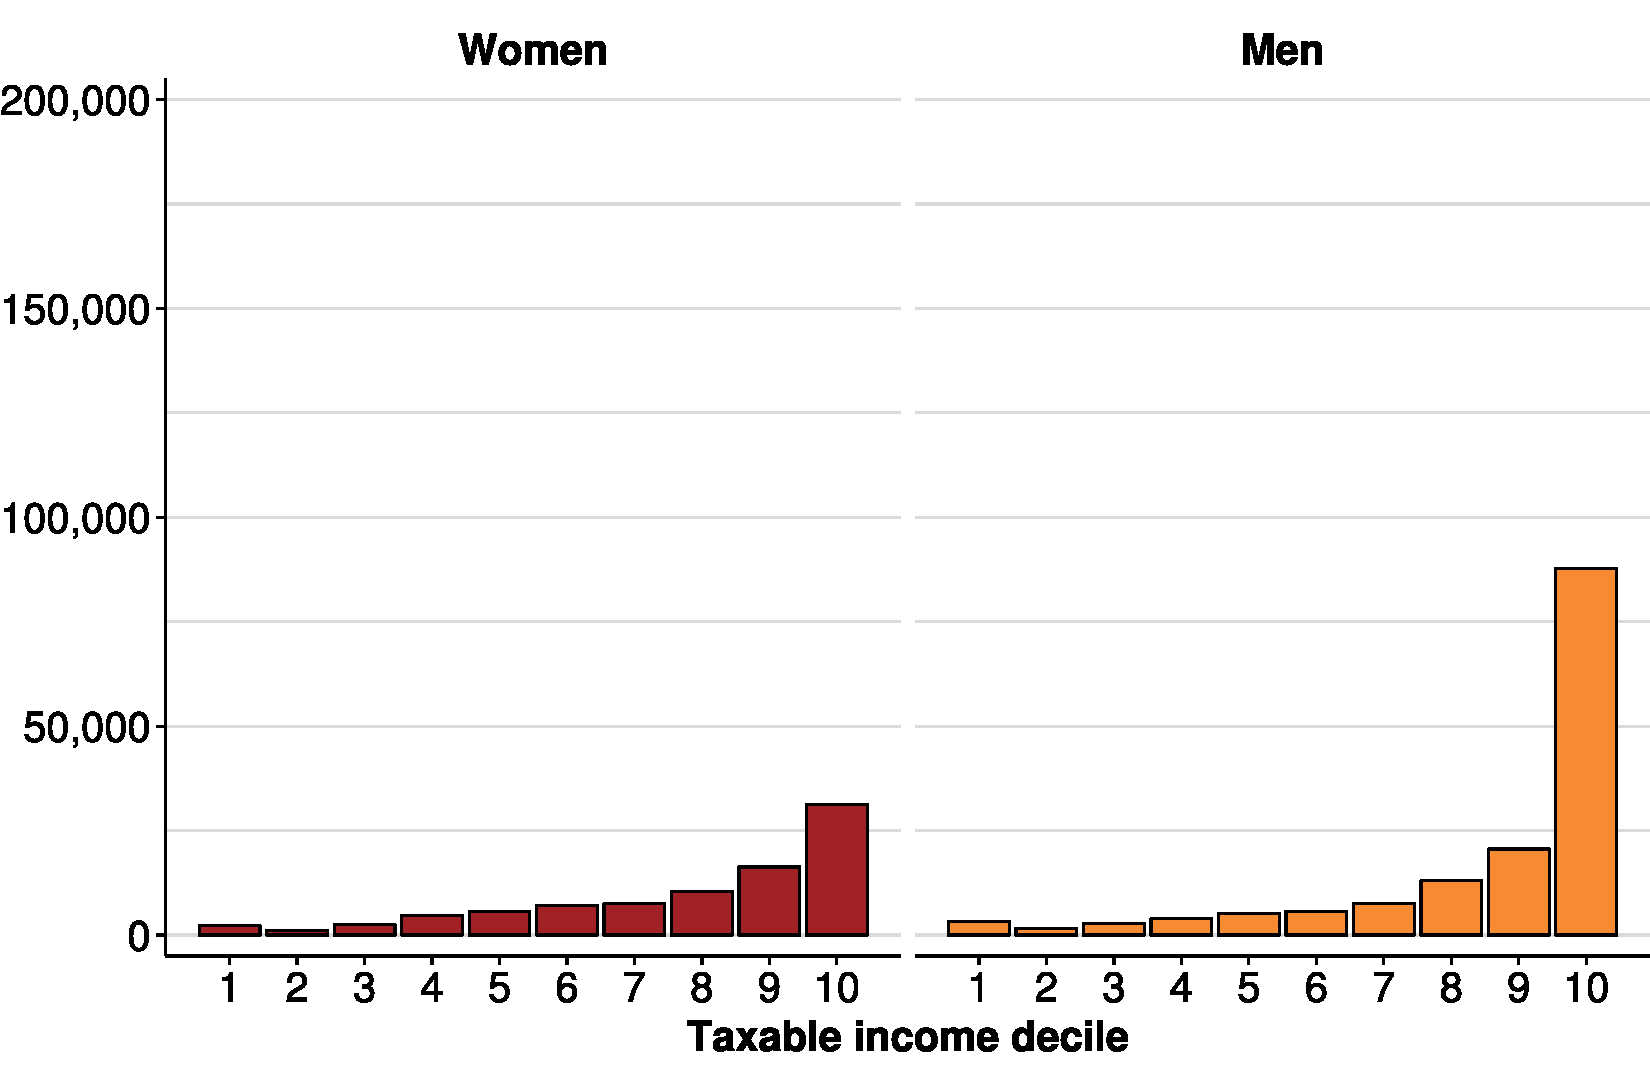
\includegraphics[width=4.47222in,height=2.94759954545455in]{figure/n-individuals-by-decile-over-500k-and-over-25k-201718-1} 

\noteswithsource{See \Cref{fig:pre-tax-contributions-25k-by-decile-201718}.}{Grattan analysis of \textcite{ATO2016SampleFile1314}.}
\end{figure}

\chapter{Future changes\label{chap:future-changes}}
Overall, both the Government’s and the ALP’s proposed changes are a big step in the right direction. 
Those affected are overwhelmingly high-income earners who are unlikely to ever qualify for the Age Pension in retirement. 
Yet the changes don’t go far enough.

\section{Super tax breaks remain poorly targeted overall even after 2016 Budget reforms}\label{sec:super-tax-breaks-remain-poorly-targeted-overall-even-after-2016-budget-reforms}

Even after the reforms, super tax breaks will overwhelmingly flow to high-income earners who do not need them. 
People in the top 20 per cent of income earners, who are unlikely to ever get a pension, will still receive about half of all super pre-tax contribution tax breaks.

Treasury projections in the 2016 Budget show that the lifetime value of tax breaks to high-income men remains much higher than the value of the Age Pension for low-income earners, even after the Government's Budget changes (\Vref{fig:npv-total-govt-lifetime-support-through-Age-Pension-super-tax}). % 
These projections are likely to be conservative since they ignore all post-tax super contributions, which are largely made by high-income earners, boosting the super earnings tax breaks they receive.\footnote{Different assumptions about life expectancy and draw down rates can also result in much higher estimates of the lifetime benefits to high-income earners. For example, \textcite{Industry-Super-2015-Off-target-current-settings} calculates that superannuation tax breaks for the top 5 per cent of income earners are worth more than \$2~million for men over their lifetimes.}

\begin{figure}[!b]
\captionwithunits{Lifetime income support is unequally distributed even after the Government's changes\label{fig:npv-total-govt-lifetime-support-through-Age-Pension-super-tax}}%
{Net present value of total government support over a lifetime through the Age Pension and super tax breaks in 2016}%


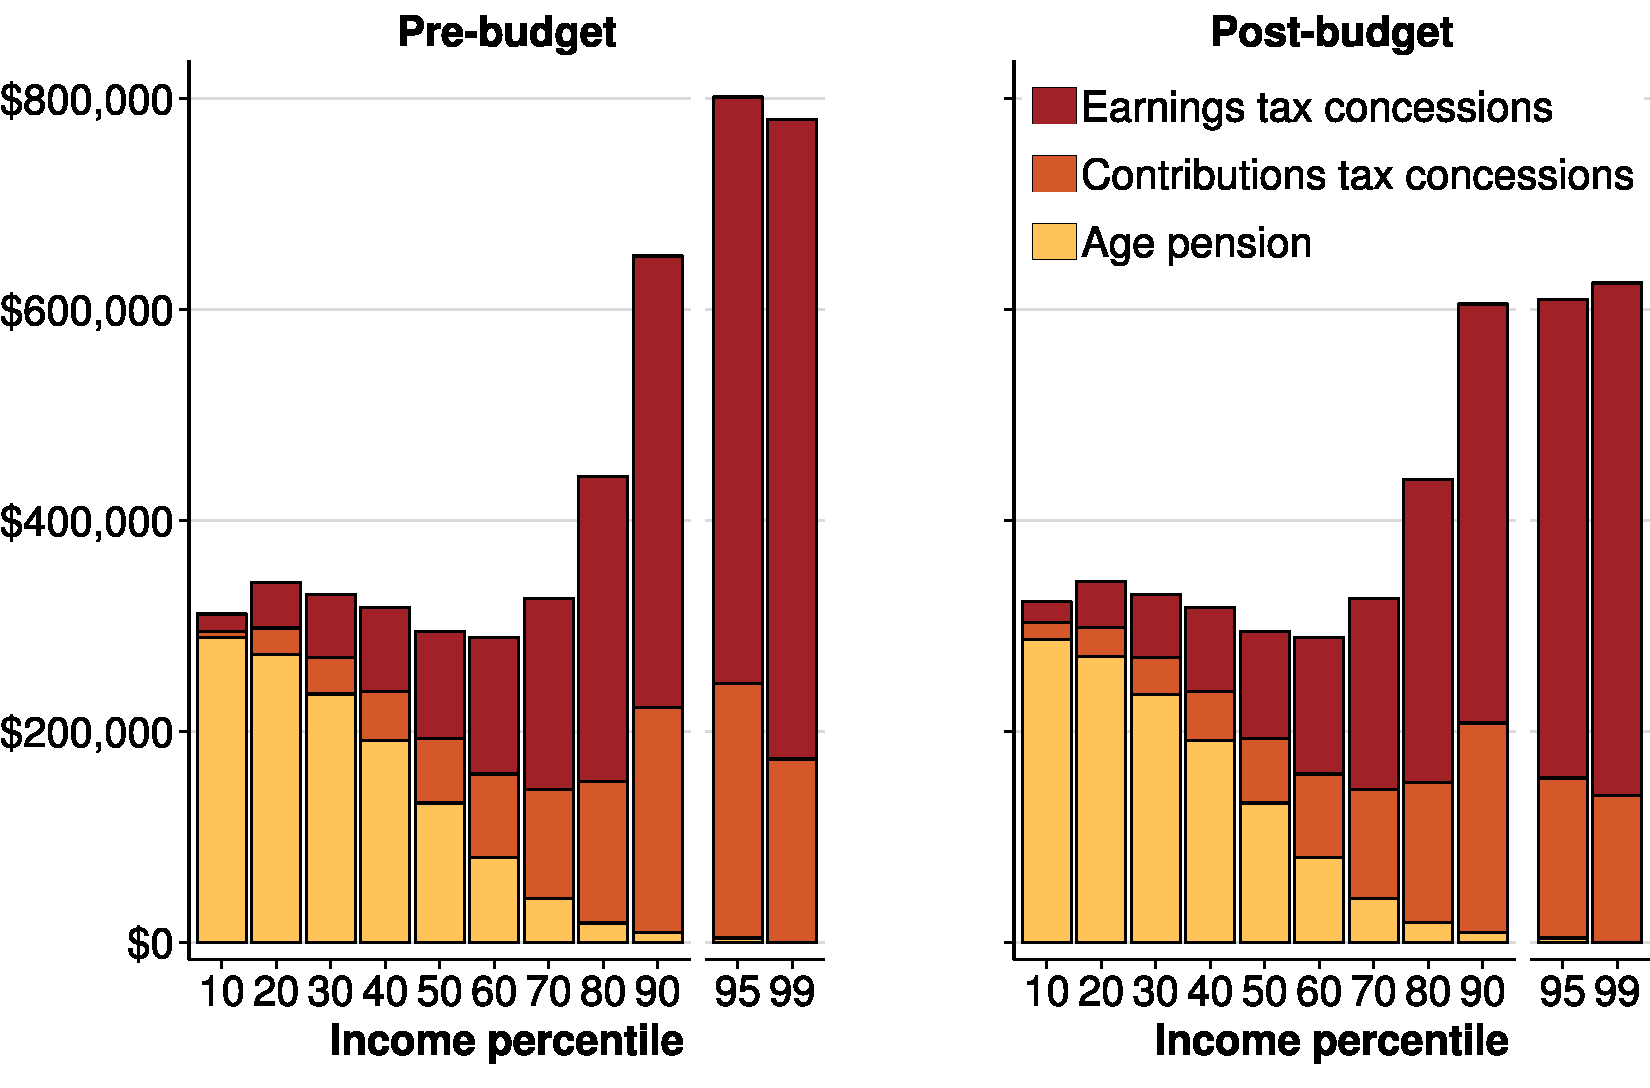
\includegraphics[width=4.47222in,height=2.94759954545455in]{figure/npv-total-govt-lifetime-support-throught-Age-Pension-super-tax-cowplot-1} 



% {Individuals are assumed to commence work in 2016 at age 30 and work until age 70, with a predicted life expectancy of 92.
% Accumulated superannuation benefits are invested in an account-based pension and individuals are assumed to draw down their assets at the current age based minimum drawdown rates.
% The level of tax assistance and Age Pension entitlements are discounted by 5 per cent per annum to calculate a net present value in 2016 dollars.
% Annual incomes are calculated for each percentile based on the distribution of earners at each single year of age.
% Assumes no non-concessional contributions}%
\noteswithsource{Individuals are assumed to commence work in 2016 at age 30 and work
until age 70, with a predicted life expectancy of 92. Accumulated superannuation
benefits are invested in an account-based pension and individuals are assumed
to draw down their assets at the current age-based minimum drawdown rates.
The level of tax assistance and Age Pension entitlements are discounted by 5
per cent per annum to calculate a net present value in 2016 dollars. Annual
incomes are calculated for each percentile based on the distribution of earners at
each single year of age. Assumes no post-tax contributions.}%
{\textcite[][4]{Budget-2016-17-Super-fact-sheets}.}
\end{figure}

Before the changes, someone in the top 1 per cent of income earners could expect to receive \textbf{two-and-a-half times as much} in tax breaks from super over her lifetime as a retiree with no assets receives in pension. 
This is also two-and-a-half times as much as the average income earner receives in pension and super tax breaks combined. 
The Budget changes merely trim the worst of these excesses: the top one per cent now receives \textbf{just twice as much} as low or average income earners.

There is no public consensus on how government support for people's retirement should be distributed. 
Yet when self-funded retirees receive twice as from government as the assistance provided by the pension, it is clear more work is required to align super tax breaks with their policy purpose.

% \chapter{Chapter with figure on same page}
\chapter{{Proposed reforms to earnings tax breaks}}\label{chap:proposed-reforms-to-earnings-tax-breaks}

\section{The \$1.6~million cap on tax-free super earnings in retirement improves targeting}\label{sec:the-1.6-million-cap-on-tax-free-super-earnings-in-retirement-improves-targeting}
For most people, income earned by their superannuation account is taxed at 15 per cent, and capital gains earned by the account at 10~per cent. 
Once people turn 60 and retire, they can move their superannuation accounts into pension phase, and then pay \emph{no} tax on the earnings.\footcite[][13]{DaleyCoatesWoodEtAl2015Super} 
The tax-free status of super earnings in retirement is a carry-over from a world in which most superannuation withdrawals were taxed.\footnote{See footnote~\ref{footnote:Simple-super-reforms} on \cpageref{footnote:Simple-super-reforms}.}

The Government’s 2016 Budget proposes to tax some of the earnings of very large superannuation accounts in pension phase. 
The proposal would only allow retirees to transfer \$1.6~million into tax-free pension accounts.\footcite[][25]{BudgetPapers201617} %  
Any superannuation balance above this threshold would remain in the “accumulation phase” where 15~per cent tax is paid on earnings. 
The proposal is expected to save \$750~million a year by 2019-20, and much more going forward.\footcite[][25]{BudgetPapers201617}
The ALP also supports this change,\footcite{Bowen-2016-Labors-plan-for-super-not-retrospective}  having previously proposed a variant of this policy that would tax annual super earnings in excess of \$75,000 at 15~per cent.\footcite{ALP2015FairerSuper} 

\begin{figure}
\captionwithunits{The 15 per cent earnings tax on super balances of more than \$1.6~million will only affect high-income earners\label{fig:super-earnings-for-60yo-in-drawdown-phase-201718}}%
{Average superannuation earnings for 60+ year olds in drawdown phase, 2017\nobreakdash-18 projection}%

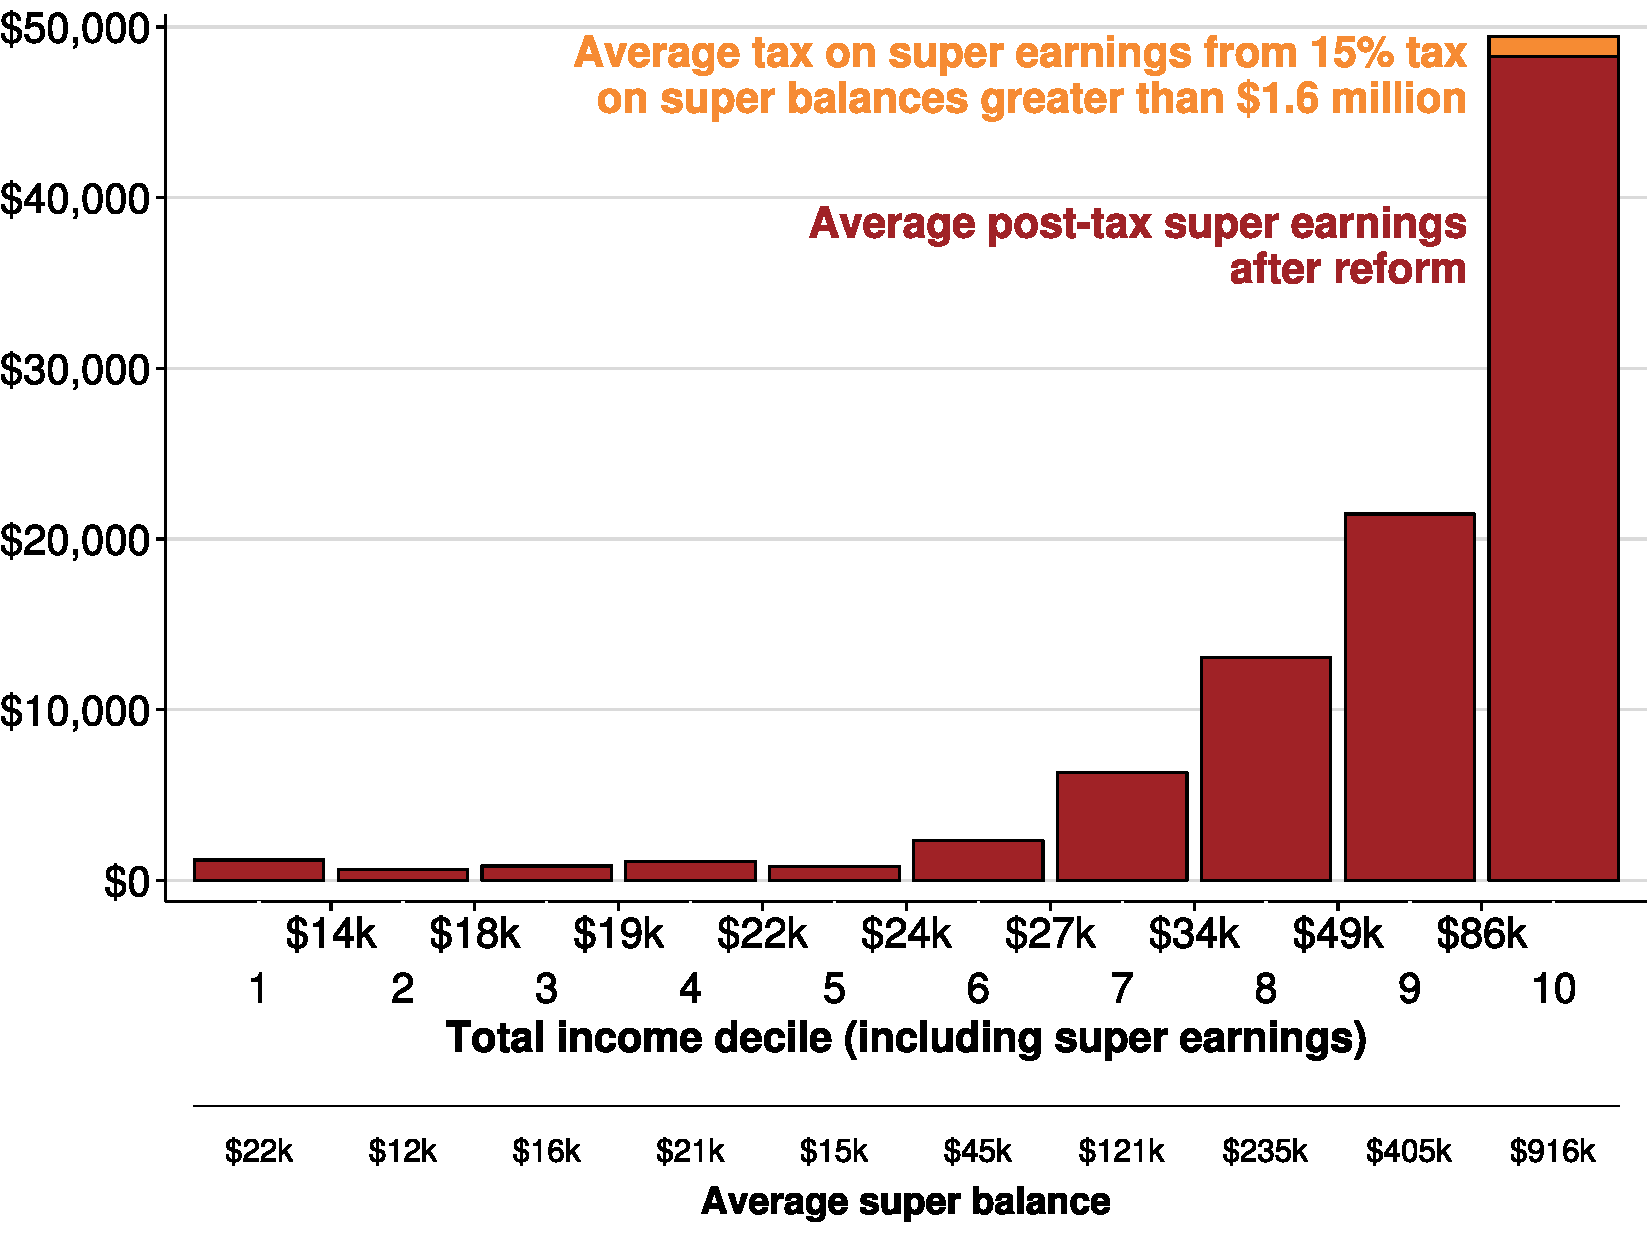
\includegraphics[width=4.47222in,height=3.38973947727273in]{figure/15pc-tax-free-earnings-noQC-1} 

%\noteswithsource{Total income \dots [excluded to fit figure].}%
%{\textcite{ABS-SIH11-CURF}.}
\end{figure}

The \$1.6~million cap on tax-free super balances in retirement would better target earnings tax breaks towards the purpose of the superannuation system.
Tax-free super earnings are a poor way to boost the retirement incomes of low and middle-income Australians.
Previous research by Grattan Institute showed that tax breaks for superannuation fund earnings are especially poorly targeted.
Two-thirds of superannuation earnings tax concessions for those aged over 60 go to the 20 per cent whose annual incomes are above \$87,000.%
\footcite[][60]{DaleyCoatesWoodEtAl2015Super} %
The cost of tax-free super earnings for retirees is \$2.7~billion a year, and will grow as more people retire with larger super balances.



The change affects only 60,000~people, all of whom are among the wealthiest 10~per cent of people aged over~60.\footnote{\label{footnote:n-affected-earnings-tax-in-retirement}%
  Grattan analysis of \textcite{ABS-SIH11-CURF}, as per \Cref{fig:super-earnings-for-60yo-in-drawdown-phase-201718}. % 
  This estimate accords with that made by \textcite{PBO-2015-Leyonhjelm-super-costing} suggesting 60,000 people would be affected by a proposal to tax super earnings in retirement exceeding \$75,000 a year at 15~per cent in 2017-18, which would affect super accounts exceeding \$1.5~million assuming a 5 per cent rate of return. 
  \textcite{ATO2016SampleFile1314} suggests up to 98,000 taxpayers aged 60~years and over had super balances exceeding \$1.6~million in 2013-14, 
  around one-third of whom would be yet to retire in 2017-18 and would thus be unaffected by the proposed earnings tax. 
  While some self-funded retirees may not submit personal income tax returns (since super withdrawals are tax-free), most retirees with balances exceeding \$1.6~million have significant other savings outside of super, and are therefore likely to submit returns. \textcite[][28]{DaleyCoatesWoodEtAl2015Super}.% 
}   This group typically has more assets outside than inside super.\footcite[][28]{DaleyCoatesWoodEtAl2015Super}  
Their assets disqualify them from getting a pension as \$1.6~million~in super exceeds the asset limit that will apply from 2017 for a part Age Pension -- \$541,250 for a single, or \$814,250 for a home-owning couple.\footcite{DHS-2016-Asset-test}

Some argue that a \$1.6~million cap on tax-free super earnings will be too low to provide adequate income in retirement.\footcite{McCrann-scott-morrison-super-changes-big-positive-deal}  
But the \$1.6~million cap is not a restriction on the amount of super that can be accumulated, it is merely a limit on the amount retirees can have before paying \emph{any} tax on their super earnings. %
Those affected would pay only a fraction of their total income in tax (\Vref{fig:super-earnings-for-60yo-in-drawdown-phase-201718}). 
For example, someone with \$2~million of assets in super would only pay \$3000~a year in tax. 

Given the tax-free threshold outside of super, a single retiree can have a combined \$2.2~million in assets in and outside the superannuation system before they pay a cent of tax.\footnote{Accounting for the tax-free threshold, Low Income Tax Offset, and the Seniors and Pensioners Tax Offset (only available to Australians aged 65 years and over).}  
The super industry itself believes that a \$545,000 asset balance is enough to provide a home-owning single person with a comfortable retirement, or \$640,000 for a couple.\footcite{ASFA2015} 

\addchap{Recommendations}
\addsec{Economic growht priorities}
\subsection*{Increasing the efficiency of taxation}

\begin{itemize}
\item Encourage the States to replace stamp duties with general
property taxes.
\item Consider lowering effective company tax rates with investment
allowances or accelerated depreciation on new investment.
\item Reduce income taxes by broadening the GST base and/or
increasing the GST rate
\item Reduce the capital gains tax discount to 25 per cent so that
other taxes can be reduced (or not raised)
\item Limit negative gearing so that passive investment losses can
only be written off against other investment income
\item In the longer term, align the tax treatment across different
types of savings by reducing taxes on other savings income
such as net rental income and bank deposits.
\end{itemize}

\nocite{long-url}
\printbibliography

\blinddocument

\the\baselineskip

\end{document}